\documentclass{standalone}
\usepackage{tikz}
\usepackage{pgfplots}
\pgfplotsset{compat=1.18}

\begin{document}
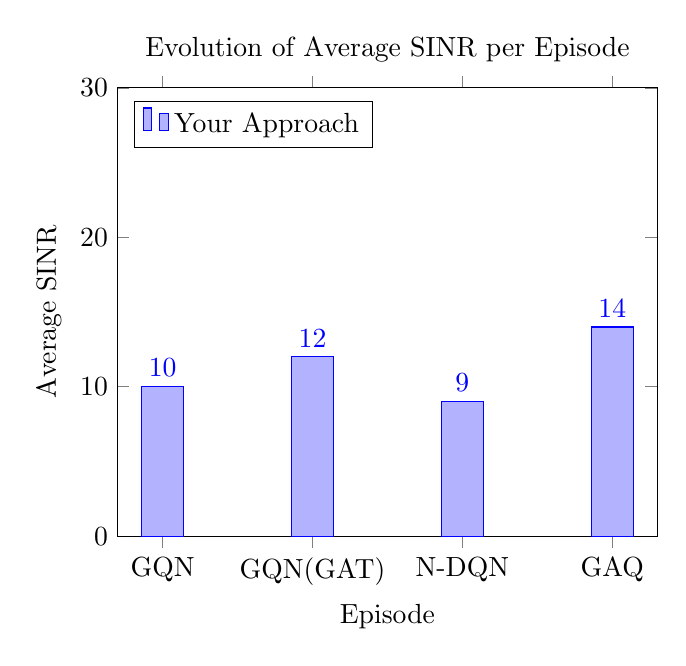
\begin{tikzpicture}
    \begin{axis}[
        title={Evolution of Average SINR per Episode},
        xlabel={Episode},
        ylabel={Average SINR},
        legend pos=north west,
        ybar,
        bar width=15pt,
        symbolic x coords={GQN, GQN(GAT), N-DQN, GAQ},
        xtick=data,
        nodes near coords,
        nodes near coords align={vertical},
        ymin=0,
        ymax=30
    ]
        \addplot coordinates {(GQN, 10) (GQN(GAT), 12) (N-DQN, 9) (GAQ, 14)};
        \legend{Your Approach, Your Approach with GAT, Standard DQN, State-of-the-Art Algorithm}
    \end{axis}
\end{tikzpicture}
\end{document}